\section{公式、图片、表格与伪代码}
本节简单介绍如何本模版下插入公式、图片、表格与伪代码。
\subsection{公式}

公式可以分为行内公式与独立公式。行内公式是指公式与文字在同一行,独立公式是指公式与文字不在同一行。行内公式使用\$包围,独立公式使用\$\$或者$\backslash [ \backslash]$包围。比如下面的代码:

\begin{lstlisting}
设有对称矩阵的SVD分解为$\mathbf{X}=\mathbf{U}\mathbf{S}\mathbf{U}^{\mathrm{T}}$,那么
\[
    \mathbf{X}^{2} = \mathbf{U} \mathbf{S}^{2} \mathbf{U}^{\mathrm{T}}.
\]
\end{lstlisting}
对应的编译结果为:
\begin{shaded}
设有对称矩阵的SVD分解为$\mathbf{X}=\mathbf{U}\mathbf{S}\mathbf{U}^{\mathrm{T}}$,那么
\[
    \mathbf{X}^{2} = \mathbf{U} \mathbf{S}^{2} \mathbf{U}^{\mathrm{T}}
\]
\end{shaded}
如果需要对公式进行编号,可以使用$\backslash \text{begin\{equation\}} \dots \backslash \text{end\{equation\}}$包围公式,比如下面的代码:
\begin{lstlisting}
设有对称矩阵的SVD分解为$\mathbf{X}=\mathbf{U}\mathbf{S}\mathbf{U}^{\mathrm{T}}$,那么
\begin{equation}
    \mathbf{X}^{2} = \mathbf{U} \mathbf{S}^{2} \mathbf{U}^{\mathrm{T}}.
    \label{eq:1}
\end{equation}
\end{lstlisting}
其中$\backslash \text{label}$为公式的标签,在引用时会用到,具体的引用方法会在后面介绍。这段代码对应的编译结果为:
\begin{shaded}
设有对称矩阵的SVD分解为$\mathbf{X}=\mathbf{U}\mathbf{S}\mathbf{U}^{\mathrm{T}}$,那么
\begin{equation}
    \mathbf{X}^{2} = \mathbf{U} \mathbf{S}^{2} \mathbf{U}^{\mathrm{T}}.
    \label{eq:1}
\end{equation}
\end{shaded}


需要注意的是,一般矩阵需用大写字母,并且为加粗正体,即$\backslash \text{mathbf}$来修饰,例如$\mathbf{X},\mathbf{A}$。而向量使用小写字母,加粗斜体表示,在本模版中定义了$\backslash \text{bm}$指令来修饰向量,例如$\bm{x},\bm{a}$。

\subsection{图片}
图片的插入使用$\backslash \text{includegraphics}$指令,不过插入单张图片和多张图片的代码是不同的。插入单张图片的代码如下:
\begin{lstlisting}
\begin{figure}[htb!]
    \centering
    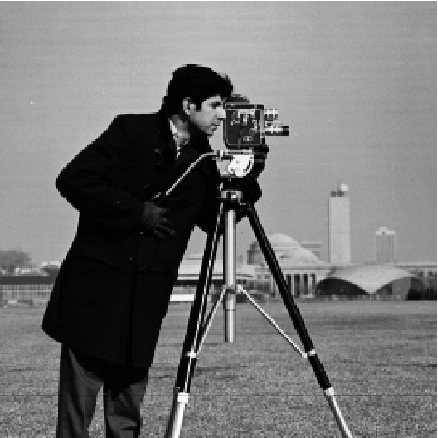
\includegraphics[width=0.3\textwidth]{./img/im1.pdf}
    \caption{一幅图片}
    \label{fig:1}
\end{figure}
\end{lstlisting}

\begin{figure}[htb!]
    \centering
    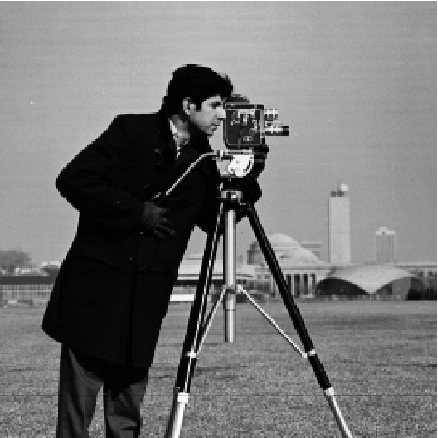
\includegraphics[width=0.3\textwidth]{./img/im1.pdf}
    \caption{一幅图片}
    \label{fig:1}
\end{figure}

插入多张图片的代码如下:

\begin{lstlisting}
\begin{figure}[htbp!]
    \centering
    \begin{subfigure}{.3\textwidth}
        \centering
        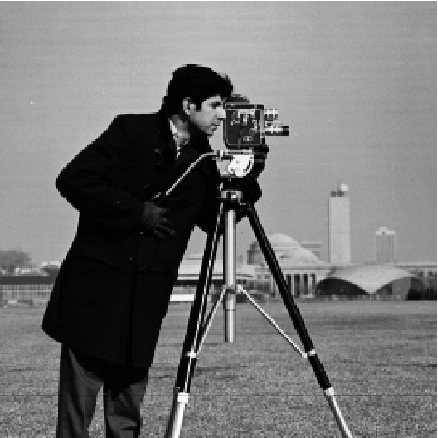
\includegraphics[width=.\textwidth]{./img/im1.pdf}
        \caption{}
        \label{fig:cameraman2_1}
    \end{subfigure}
    \begin{subfigure}{.3\textwidth}
        \centering
        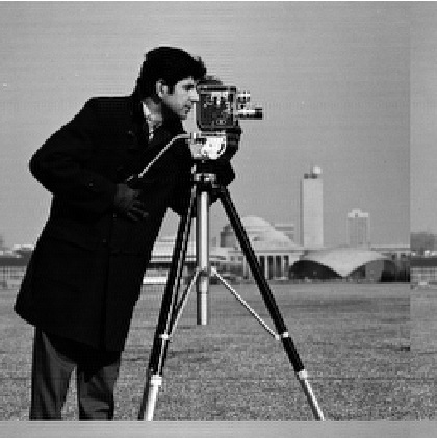
\includegraphics[width=.\textwidth]{./img/im2.pdf}
        \caption{}
        \label{fig:cameraman2_2}
    \end{subfigure}
    \caption{两幅图片 (a) 原图像 (b) 平移后的图像}
    \label{fig:cameraman2}
\end{figure}
\end{lstlisting}

\begin{figure}[htb!]
    \centering
    \begin{subfigure}{.3\textwidth}
        \centering
        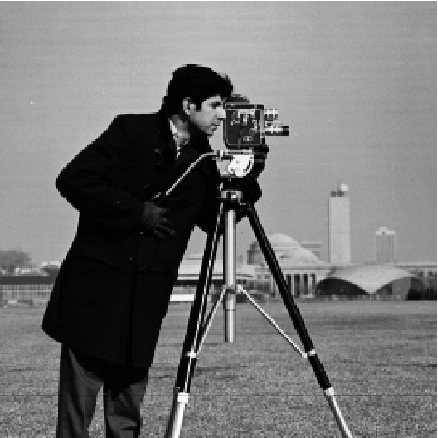
\includegraphics[width=\textwidth]{./img/im1.pdf}
        \caption{}
        \label{fig:cameraman2_1}
    \end{subfigure}
    \begin{subfigure}{.3\textwidth}
        \centering
        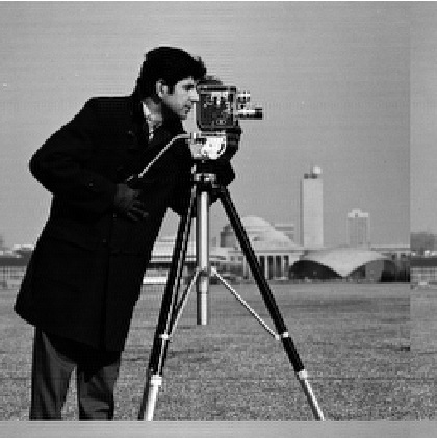
\includegraphics[width=\textwidth]{./img/im2.pdf}
        \caption{}
        \label{fig:cameraman2_2}
    \end{subfigure}
    \caption{两幅图片 (a) 原图像 (b) 平移后的图像}
    \label{fig:cameraman2}
\end{figure}

\subsection{表格}
